% =============================================================================
% Explainable Hybrid ASAG — full-length journal manuscript (Q2/Q3-ready, generic).
% Compiles with the stock `article` class; swap the preamble for the venue
% template at submission (section structure and \cite keys carry over).
% Build: pdflatex main && bibtex main && pdflatex main && pdflatex main
%
% STATUS: all numbers are verified against reports/** as of 2026-07-04 (v2).
%   Hybrid (DeBERTa) results are PENDING the Colab run — every pending value
%   is marked \TBD{...}. Search for "TBD" before submission.
% =============================================================================
\documentclass[11pt]{article}
\usepackage[margin=1in]{geometry}
\usepackage{graphicx}
\usepackage{booktabs}
\usepackage{amsmath}
\usepackage{multirow}
\usepackage{url}
\usepackage[hidelinks]{hyperref}
\graphicspath{{../reports/figures/}}

% ---- pending-result marker (remove all before submission) ----
\newcommand{\TBD}[1]{\textbf{[TBD: #1]}}

\title{Leakage-Aware, Interpretable Feature Fusion for Automatic Short Answer
Grading across Heterogeneous Datasets}
\author{Ashraf Kahlout\\ \small Affiliation --- to be added}
\date{}

\begin{document}
\maketitle

\begin{abstract}
Automatic short answer grading (ASAG) systems are increasingly accurate but
opaque, and their reported accuracy is often inflated by an under-examined
evaluation artifact: when answers to the same \emph{question} appear in both
training and test folds, models exploit question-specific shortcuts rather than
genuine answer understanding. We present (i)~a systematic \textbf{question-leakage
audit} across six heterogeneous ASAG datasets, (ii)~an interpretable
feature-fusion grader---a NaN-native gradient-boosted head over lexical,
semantic, and rubric-coverage feature branches---and (iii)~an explainability
study whose attributions are validated against pre-existing human gold feedback.
Replacing the still-common stratified $k$-fold protocol with grouped
leave-questions-out cross-validation collapses apparent performance by up to
38~macro-F1 points (Powergrading $0.830\!\rightarrow\!0.450$), and a control
model that sees \emph{only} the question identity nearly matches the full model
under the leaky protocol ($0.873$ vs.\ $0.830$). Under the honest protocol, our
tuned head beats trivial and question-shortcut baselines on four of six
datasets, with significance established by a cluster bootstrap over questions
under Holm correction---a procedure that reverses two apparent wins that an
item-level bootstrap would have accepted. Branch ablations show hand-crafted
linguistic features remain the accuracy workhorse, while the rubric branch is
\emph{faithful but accuracy-neutral}: its concept-coverage signals rise
monotonically with human verdicts on the SAF corpus (AUC up to $0.62$),
providing teacher-style explanations at no accuracy cost. We further report
calibration (temperature scaling halves SemEval ECE, $0.122\!\rightarrow\!0.059$),
perturbation robustness, and leave-one-dataset-out transfer.
% TODO(after Colab run): add one sentence with the hybrid three-way headline.
A DeBERTa cross-encoder arm, fused as an out-of-fold feature that preserves
exact TreeSHAP attributions, is evaluated under identical unseen-question folds
(\TBD{hybrid headline sentence after Colab run}). All code, splits, and reports
are released.
\end{abstract}

\medskip
\noindent\textbf{Keywords:} automatic short answer grading; educational NLP;
evaluation methodology; data leakage; explainable AI; SHAP; calibration;
gradient boosting; transformers

\section{Introduction}
\label{sec:intro}

Short answer grading asks a model to score a free-text student response against
a question and, usually, a reference answer. The task sits between paraphrase
detection, textual entailment, and ordinal regression
\cite{burrows2015eras,dzikovska2013semeval}, and a deployed grader must be both
accurate \emph{and} auditable by the teacher who signs the grade. Two problems
motivate this work.

\paragraph{Evaluation honesty.}
Several widely used ASAG corpora (Mohler \cite{mohler2011learning},
Powergrading \cite{basu2013powergrading}, MIND-CA \cite{kovatchev2020mind})
ship without official train/test splits, so practitioners fall back on
stratified $k$-fold cross-validation over answers. But if one question's
answers are distributed across folds, the model can memorize
question-specific regularities---the answer distribution, typical phrasing,
even answer length---and these shortcuts \cite{geirhos2020shortcut} vanish on
genuinely new questions. The community has long known that unseen-question
generalization is harder (SemEval-2013 defined unseen-answer/question/domain
test sets a decade ago \cite{dzikovska2013semeval}; Condor et al.\ showed the
drop directly for SBERT graders \cite{condor2021automatic}), yet the leaky
protocol remains common practice, and \emph{how much} it inflates published-style
numbers on these standard corpora has not been quantified. We quantify it, with
a diagnosis (between-question variance share), a control (a model that sees
only the question identity), and a remedy (grouped leave-questions-out CV).

\paragraph{Interpretability.}
High-capacity encoders grade well but cannot tell a teacher \emph{why} a mark
was given, and post-hoc explanations of black-box graders are rarely validated
against human judgment \cite{poulton2021explaining,tornqvist2023exasag}. A
fusion grader whose inputs are human-readable (overlap, negation, concept
coverage) admits exact per-feature attributions via TreeSHAP
\cite{lundberg2017unified,lundberg2020local}; the question is whether those
attributions actually track what human graders reward. The SAF corpus
\cite{filighera2022your} uniquely ships per-answer human verification feedback,
which we use as a \emph{pre-existing} gold standard for explanation validation
---no new annotation required.

\paragraph{Research questions.}
\begin{itemize}
  \item \textbf{RQ1} (leakage): How much does question-level leakage inflate
        ASAG results under stratified $k$-fold CV, and what remains under
        grouped leave-questions-out evaluation?
  \item \textbf{RQ2} (branches): Which interpretable feature branches
        (semantic, linguistic, rubric-coverage) carry the accuracy, and what do
        negation-scope cues add?
  \item \textbf{RQ3} (explanations): Are the head's explanations faithful to
        the model, and do the interpretable signals align with human gold
        feedback?
  \item \textbf{RQ4} (deployment): How calibrated and perturbation-robust is
        the grader, and does anything transfer across datasets?
  \item \textbf{RQ5} (hybrid): Does an out-of-fold transformer signal, fused as
        one more feature, improve unseen-question accuracy while preserving
        exact attributions? \TBD{answered after the Colab run}
\end{itemize}

\paragraph{Contributions.}
(1)~A question-leakage audit across six heterogeneous ASAG datasets, pairing a
seen-question upper bound with an honest grouped protocol and a
question-shortcut control baseline (Section~\ref{sec:protocol},
Table~\ref{tab:leakage}); (2)~an interpretable, NaN-native feature-fusion
grader evaluated across classification, ordinal, and regression targets with
per-dataset Optuna tuning that never touches test data
(Section~\ref{sec:method}); (3)~branch ablations isolating each feature
family's contribution under the honest protocol (Table~\ref{tab:ablations});
(4)~an explainability study combining exact TreeSHAP, a faithfulness
decomposition, rubric concept attribution, and validation against SAF's human
gold feedback (Section~\ref{sec:results-xai}); (5)~a cluster-bootstrap
significance analysis with Holm correction that reverses two apparent wins
(Table~\ref{tab:sig}); (6)~calibration, robustness, and leave-one-dataset-out
transfer analyses (Sections~\ref{sec:results-robust}--\ref{sec:results-lodo});
and (7)~a hybrid arm fusing out-of-fold DeBERTa signals into the same
interpretable head under identical folds (Section~\ref{sec:results-hybrid},
\TBD{pending}). Code, splits, and all report artifacts are released for
reproduction.

\section{Related Work}
\label{sec:related}

\subsection{Automatic short answer grading}
ASAG has evolved from hand-engineered similarity features
\cite{mohler2011learning,sultan2016fast,burrows2015eras} through the
SemEval-2013 shared task \cite{dzikovska2013semeval} to neural scorers
\cite{riordan2017investigating} and transformer fine-tuning
\cite{sung2019improving,sung2019pretraining,camus2020investigating}. Surveys
note that the strongest reported systems often combine hand-crafted features
with transformer semantics \cite{haller2022survey}, and a scoping review finds
the marginal contribution of embeddings over conventional features inconclusive
\cite{putnikovic2023embeddings}---both observations motivate keeping an
interpretable feature core. Similarity-based (reference-comparison) scoring has
been defended as more classroom-suitable than instance-based scoring because it
transfers to new questions with few labels \cite{bexte2022similarity,
bexte2023similarity}; our rubric and semantic branches follow that design.
ASAG2024 recently unified seven corpora into a combined benchmark
\cite{meyer2024asag2024}; we share the multi-dataset spirit but keep each
dataset's native target and metric, adding protocol-level auditing instead of
scale unification.

\subsection{Evaluation protocols and question leakage}
SemEval-2013 institutionalized unseen-answer (UA), unseen-question (UQ), and
unseen-domain (UD) test sets \cite{dzikovska2013semeval}, and SAF ships UA/UQ
splits \cite{filighera2022your}. Condor et al.\ compared random vs.\
question-level holdouts for SBERT-based ASAG and observed sharp drops
\cite{condor2021automatic}; recent datasets quantify the same cliff
\cite{aggarwal2024engsaf}. In essay scoring, Li and Ng re-examined cross-prompt
evaluation and found simple feature-based models match neural state of the art
once prompts are properly held out \cite{li2024conundrums}. Our audit differs
in three ways: it targets the \emph{no-official-split} ASAG corpora where
stratified $k$-fold remains the default, it reports the inflation explicitly as
a seen-vs-grouped gap with a question-identity-only control model, and it pairs
the audit with variance diagnostics ($\eta^2$) that predict which datasets are
most leakage-prone. To our knowledge no prior work publishes such an audit for
Mohler, Powergrading, and MIND-CA. Shortcut learning is the general framing
\cite{geirhos2020shortcut}.

\subsection{Explainable ASAG}
Post-hoc attribution methods have been applied to transformer graders
\cite{poulton2021explaining}, and ExASAG generates natural-language
explanations validated against recruited experts \cite{tornqvist2023exasag}.
AERA distills LLM rationales into a smaller scoring-plus-explaining model
\cite{li2023distilling}. Our approach is complementary and cheaper: the model
is interpretable \emph{by construction} (31 human-readable features), the
attributions are exact rather than approximate \cite{lundberg2020local}, and
validation uses SAF's \emph{pre-existing} human verification feedback rather
than newly collected judgments---turning a shipped dataset field into a free
gold standard for explanation quality.

\subsection{Hybrid feature--transformer graders}
GradeAid concatenates TF--IDF features with BERT cross-encoder similarity for
regression heads across public ASAG corpora \cite{delgobbo2023gradeaid};
hybrid feature-plus-embedding ensembles are likewise common in essay scoring.
Our hybrid differs in the evaluation and explanation contract: the transformer
signal enters as an \emph{out-of-fold} prediction (never fit on its own test
fold), the fusion head remains NaN-native gradient boosting with exact TreeSHAP,
and neural-only / feature-only / hybrid arms are compared under identical
grouped unseen-question folds. \TBD{tighten this paragraph once hybrid numbers
exist}

\subsection{LLM-era grading}
Zero- and few-shot LLM graders are attractive but currently unreliable as sole
graders: they trail fine-tuned or classical supervised systems on agreement
metrics \cite{chamieh2024llms}, and GPT-4-with-prompting has been reported to
lose to traditional models in recent head-to-heads \cite{ferreiramello2025gpt4}.
Rationale-distillation improves over raw ChatGPT scoring \cite{li2023distilling}.
Our contribution is orthogonal: an audited evaluation protocol and a validated,
CPU-only, transparent head that institutions can run locally; the protocol
itself applies unchanged to LLM graders.
% TODO(optional, high value): add a zero-shot LLM row to Table main and cite it here.

\subsection{Robustness, calibration, and deferral}
Adversarial studies show ASAG systems can be fooled by universal triggers and
even adjective/adverb insertion \cite{filighera2020fooling,filighera2023cheating,
ding2020dont}, motivating perturbation testing. Confidence estimation for
routing uncertain answers to humans was proposed for Japanese SAS
\cite{funayama2020preventing} and extended to human-in-the-loop cost analyses
\cite{funayama2022balancing}. We follow temperature scaling
\cite{guo2017calibration} for calibration and report risk--coverage curves;
our significance methodology follows the cluster (block) bootstrap
\cite{efron1993bootstrap} with Holm--Bonferroni control \cite{holm1979simple}.

\section{Datasets and Task Formulation}
\label{sec:data}

Every loader emits one unified schema
(\texttt{question\_id}, \texttt{question}, \texttt{reference\_answer},
\texttt{student\_answer}, \texttt{score}, \texttt{label}, \texttt{dataset},
\texttt{domain}, \texttt{split}), enforced by tests. The six datasets
(Table~\ref{tab:data}) deliberately span three task types---5-way
classification, ordinal, bounded regression---three split regimes, and five
subject domains. Two datasets (ASAP-SAS, MIND-CA) provide no reference answer,
so 24 of 31 reference-dependent features are intentionally \texttt{NaN} there
and ignored natively by the tree head (no imputation). For corpora without
official splits, exact duplicate answers within a question are collapsed to the
median-score row before splitting (Powergrading $13{,}960\!\rightarrow\!4{,}941$;
MIND-CA $11{,}311\!\rightarrow\!10{,}543$; Mohler $1{,}260\!\rightarrow\!616$),
removing a trivial memorization vector. Licensing and acquisition details for
each corpus are documented in the released repository; raw data are not
redistributed.

\begin{table}[t]
\centering\small
\begin{tabular}{llllll}
\toprule
Dataset & Domain & Task / target & Questions & Answers & Split regime \\
\midrule
SemEval-2013 T7 \cite{dzikovska2013semeval} & science tutoring & 5-way clf / label & 252 & 16{,}003 & official UA/UQ/UD \\
SAF \cite{filighera2022your} & comm.\ networks & regression / score & 31 & 2{,}981 & official UA/UQ \\
ASAP-SAS \cite{hewlett2012asapsas}$^{\dagger}$ & science, biology & ordinal / QWK & 4 prompts & 8{,}722 & official train/dev/test \\
Mohler \cite{mohler2011learning}$^{\ddagger}$ & CS data structures & regression / Pearson & 21 & 616$^{*}$ & grouped CV \\
Powergrading \cite{basu2013powergrading} & US civics & binary clf / macro-F1 & 20 & 4{,}941$^{*}$ & grouped CV \\
MIND-CA \cite{kovatchev2020mind} & psychology (children) & ordinal / QWK & 11 & 10{,}543$^{*}$ & grouped CV \\
\bottomrule
\end{tabular}
\caption{Evaluation datasets. $^{*}$after within-question deduplication.
$^{\dagger}$via the AERA mirror \cite{li2023distilling}: EssaySets 1, 2, 5, 6
(4 of 10 prompts) but with gold test-split scores. $^{\ddagger}$via the
ASAG2024 subset \cite{meyer2024asag2024}: 21 of the original 80 questions.
Because Mohler and ASAP-SAS are subsets, we report internal numbers only and
make no head-to-head claims against published results
(Section~\ref{sec:results-context}).}
\label{tab:data}
\end{table}

\section{Method}
\label{sec:method}

\subsection{Two-view preprocessing}
Each row is normalized into two parallel views written to separate columns.
The \emph{encoder view} applies NFKC and whitespace normalization only,
preserving the signal transformers expect. The \emph{feature view} applies
spaCy \cite{honnibal2020spacy} lemmatization, lowercasing, and
punctuation/stopword removal \emph{with negators preserved}. A third,
negation-scope view additionally prefixes tokens inside a negator's scope
(window of 4 kept tokens, closed early at clause boundaries), so that
``does not forward'' yields \texttt{neg\_forward}; contrasting features built
from the plain vs.\ scope-marked views provides a ready-made negation ablation
(Section~\ref{sec:results-ablation}). An empirical subword token-length study
over both a WordPiece and a SentencePiece tokenizer justified
$\text{max\_len}=128$ for the encoder regime ($\le 1.09\%$ truncation on five
datasets), with a per-dataset override of 256 for SAF, whose multi-point
reference solutions are long.

\subsection{Interpretable feature branches (31 features)}
Features are grouped into three branches, each a pure function of the two
views:
\begin{itemize}
  \item \textbf{Branch A --- semantic (3):} SBERT \cite{reimers2019sentencebert}
        (all-MiniLM-L6-v2) student--reference cosine, mean absolute embedding
        difference, and mean Hadamard product.
  \item \textbf{Branch B --- linguistic (23):} token/bigram/trigram overlap,
        precision/recall/Dice variants, content-word overlap on the
        negation-marked view, length and length-ratio statistics, TF--IDF
        cosine, negation cue counts and student--reference polarity mismatch,
        and named-entity overlap statistics.
  \item \textbf{Branch C --- rubric coverage (5):} each reference-answer
        sentence is treated as a rubric concept; per-concept max SBERT
        similarity to the student answer yields mean/min/max similarity,
        concept count, and coverage@$\tau$ ($\tau{=}0.5$, fixed, untuned).
\end{itemize}
Reference-dependent features are \texttt{NaN} where no reference exists. The
full feature dictionary (definition, view, NaN conditions per feature) ships
with the code.

\subsection{Fusion head}
The head is LightGBM \cite{ke2017lightgbm}: a classifier for categorical
targets and a regressor otherwise; ordinal targets use regression followed by
rounding and clipping to the training grade range. LightGBM handles
\texttt{NaN} natively at split time, which is what makes a single 31-feature
space usable across datasets with and without reference answers. ASAP-SAS is
evaluated per prompt (one model per \texttt{EssaySet}, QWK macro-averaged),
since each prompt has its own rubric and scale.

\subsection{Hybrid arm: transformer-as-feature}
\label{sec:method-hybrid}
The hybrid does \emph{not} replace the head. A DeBERTa-v3-base
\cite{he2021deberta,he2023debertav3} cross-encoder is fine-tuned on
(reference-or-question, student answer) pairs with a task-appropriate head, and
its predictions are exported \emph{out of fold}: for grouped-CV datasets, each
fold's rows are scored by a model trained on the other folds; for
official-split datasets, test rows are scored by a model trained on the train
split, while train rows receive inner grouped-CV out-of-fold scores so the
fusion head never sees in-sample neural predictions. The exported signals
(\texttt{neural\_score}, \texttt{neural\_pred}) are concatenated to the feature
matrix as branch~D, preserving the NaN-native head and exact TreeSHAP
attributions---including the ability to measure how much attribution mass the
neural signal absorbs from the interpretable branches.
\TBD{This arm is fully implemented; numbers await the GPU run
(Section~\ref{sec:results-hybrid}).}

\subsection{Hyperparameter optimization and controls}
Per dataset, Optuna \cite{akiba2019optuna} (TPE, 40 trials, fixed sampler seed)
tunes seven LightGBM parameters (learning rate, leaves, estimators, child
samples, subsample, column subsample, $\ell_1/\ell_2$) on the official dev
split when one exists, otherwise on an inner grouped CV carved from training
rows only---\textbf{the objective never touches a test split}. Every learned
result is paired with two controls: a \emph{trivial baseline}
(majority/mean/median of train) and a \emph{question-shortcut} model that
predicts each test answer using only the training mean (or majority label) of
its question, backing off to the global statistic for unseen questions. The
question-shortcut arm is the leakage diagnosis made into a model: any score it
achieves is obtainable without reading the student's answer.

\section{Leakage-Aware Evaluation Protocol}
\label{sec:protocol}

\paragraph{Grouped leave-questions-out CV.}
For datasets without official splits we use stratified group $k$-fold
($k{=}5$) with \texttt{question\_id} as the group and binned scores as strata,
so no question ever spans train and test. Folds are materialized once and
reused by every experiment (training, HPO inner loops, ablations, XAI), and
5 seeds are reported as mean$\pm$std.

\paragraph{Seen-question upper bound and generalization gap.}
Alongside the grouped estimate we compute the legacy stratified $k$-fold as a
\emph{transient seen-question upper bound}; the difference is the leakage the
grouped protocol removes (RQ1). For official-split datasets the analogous gap
is the drop from unseen-answer to unseen-question/domain test sets.

\paragraph{Cluster-bootstrap significance with family-wise control.}
Item-level bootstraps assume independent items, but answers to one question are
correlated; resampling items overstates the effective sample size exactly on
the datasets with few questions. We therefore resample \emph{whole questions}
with replacement (10{,}000 replicates) and report the observed
$\Delta=\text{head}-\text{baseline}$, its percentile 95\% CI, and the one-sided
$p=P(\Delta\le 0)$, Holm-corrected across the six datasets
\cite{efron1993bootstrap,holm1979simple}. For the per-prompt ASAP-SAS, the
prompt is the cluster and answers are resampled within prompt. Significance is
computed on the tuned head's seed-42 predictions; multi-seed variability is
reported separately in Table~\ref{tab:main} (it is an order of magnitude
smaller than the CIs).

\paragraph{Human ceiling.}
ASAP-SAS retains a second rater on train+dev; the inter-annotator QWK
(per prompt 0.914--0.956, macro 0.942) contextualizes machine QWK as a
corpus/rubric property. The other corpora do not retain per-rater reads, which
we report as a limitation rather than approximating a ceiling.

\section{Experimental Setup}
\label{sec:setup}

All experiments are CPU-only (feature slice) with global seed 42; results
report 5 seeds (42, 1, 2, 3, 4) as mean$\pm$std. With default (untuned)
LightGBM parameters the head is deterministic (subsample and column subsample
$=1.0$), so the 5-seed std of the untuned configuration is exactly zero; tuned
configurations subsample and therefore exhibit honest non-zero seed variance.
Python 3.11; LightGBM, scikit-learn \cite{pedregosa2011scikit}, pandas
\cite{mckinney2010pandas}, spaCy, sentence-transformers; 73 unit tests cover
schema, split, feature, metric, and head contracts. Dataset downloads are
checksummed; all reports quoted here are regenerated by single \texttt{make}
targets.
% TODO: add a runtime/memory table (train + inference per dataset, CPU spec)
% before submission — numbers not yet collected.

\section{Results}
\label{sec:results}

\subsection{RQ1: The question-leakage audit}
\label{sec:results-leakage}

Table~\ref{tab:leakage} quantifies the inflation on the three corpora where
stratified $k$-fold is common practice. Two observations. First, the inflation
is large and dataset-dependent: Powergrading loses 38 macro-F1 points when
questions are held out. Second, the \emph{question-shortcut control explains
the inflation}: under the leaky protocol, a model that sees only
\texttt{question\_id} nearly matches (Mohler: 0.365 vs.\ 0.570) or even
\emph{exceeds} (Powergrading: 0.873 vs.\ 0.830) the full 31-feature model,
while under the grouped protocol it collapses to (or below) the trivial
baseline. The between-question variance share predicts vulnerability:
Powergrading's labels are almost entirely question-determined
($\eta^2{=}0.92$), MIND-CA's much less so ($\eta^2{=}0.14$), and the
inflation tracks this ordering.

\begin{table}[t]
\centering\small
\begin{tabular}{llccccc}
\toprule
& & \multicolumn{2}{c}{Full head} & \multicolumn{2}{c}{Question-shortcut} & \\
\cmidrule(lr){3-4}\cmidrule(lr){5-6}
Dataset & Metric & strat.\ (leaky) & grouped & strat.\ (leaky) & grouped & $\eta^2$ \\
\midrule
Mohler       & Pearson  & 0.570 & 0.430 & 0.365 & $-0.166$ & 0.186 \\
Powergrading & macro-F1 & 0.830 & 0.450 & \textbf{0.873} & 0.392 & 0.915 \\
MIND-CA      & QWK      & 0.121 & 0.059 & 0.164 & 0.000 & 0.141 \\
\bottomrule
\end{tabular}
\caption{Question-leakage audit (default head; \texttt{reports/phase4\_audit/}).
``Strat.'' = stratified $k$-fold with questions spanning folds (leaky);
``grouped'' = leave-questions-out. The question-shortcut model predicts from
question identity alone. $\eta^2$ = between-question share of score variance.
A lightly regularized head replicates the pattern (inflation $+0.17$, $+0.35$,
$+0.08$ respectively).}
\label{tab:leakage}
\end{table}

The official-split corpora corroborate the audit. On SemEval, the tuned head
drops from 0.508 (unseen answers) to 0.453 (unseen questions) and 0.427
(unseen domains), while the question-shortcut arm scores 0.323 macro-F1 on
unseen answers---nearly triple the majority baseline (0.118)---and collapses to
the baseline on unseen questions, as it must. SAF is the extreme case: seen
questions yield Pearson $r{=}0.904$, of which the question shortcut alone
achieves $0.891$; on unseen questions the head falls to $0.019\pm0.033$,
i.e., essentially nothing the model learned about SAF's five test-UQ questions
transfers. We therefore treat SAF as an explainability case study
(Section~\ref{sec:results-xai}) rather than an accuracy result.

\subsection{Main results under the honest protocol}
\label{sec:results-main}

Table~\ref{tab:main} reports the tuned head against both controls on each
dataset's headline split. Tuning adds modest, consistent gains over the
default head (e.g., SemEval $0.411\!\rightarrow\!0.427$; Mohler
$0.430\!\rightarrow\!0.490$; Powergrading $0.450\!\rightarrow\!0.486$). The
ASAP-SAS QWK of $0.363$ should be read against both the human ceiling
($0.942$) and the fact that only branch~B is populated (no reference answers);
the remaining gap is the direct measurement of how far interpretable
answer-side features alone are from rubric-informed human judgment on this
subset.

\begin{table}[t]
\centering\small
\begin{tabular}{llcccc}
\toprule
Dataset (headline split) & Metric & Tuned head & Default head & Trivial base & Q-shortcut \\
\midrule
SemEval (test\_ud)  & macro-F1 & $0.427\pm0.005$ & 0.411 & 0.118 & 0.118 \\
ASAP-SAS (test\_ua) & QWK      & $0.363\pm0.003$ & 0.350 & 0.000 & 0.000 \\
Mohler (grouped CV) & Pearson  & $0.490\pm0.001$ & 0.430 & --- & $-0.166$ \\
SAF (test\_uq)      & Pearson  & $0.019\pm0.033$ & 0.026 & --- & --- \\
Powergrading (grouped CV) & macro-F1 & $0.486\pm0.009$ & 0.450 & 0.392 & 0.392 \\
MIND-CA (grouped CV) & QWK     & $0.077\pm0.003$ & 0.059 & 0.000 & 0.000 \\
% TODO(after Colab run): add columns "Neural-only" and "Hybrid" here, or keep
% the three-way comparison in Table~\ref{tab:hybrid} only.
\bottomrule
\end{tabular}
\caption{Tuned head (Optuna, mean$\pm$std over 5 seeds) vs.\ default head and
controls on headline splits (\texttt{reports/phase2d/}). ``---'' = degenerate
(constant) predictor, correlation undefined. On k-fold datasets the trivial
baseline and question-shortcut coincide by construction on unseen questions.}
\label{tab:main}
\end{table}

\subsection{Significance under the cluster bootstrap}
\label{sec:results-sig}

Table~\ref{tab:sig} and Figure~\ref{fig:sig} give the cluster-bootstrap
analysis. The head's gain is significant on SemEval, ASAP-SAS, Mohler, and
MIND-CA, and \emph{not} significant on Powergrading
($\Delta{=}0.079$, $p_{\text{Holm}}{=}0.291$; only 20 questions) or SAF
($p{=}0.582$; 5 test questions). An item-level bootstrap would have declared
Powergrading significant; resampling questions is what prevents that error.
This is the statistical face of the audit in
Section~\ref{sec:results-leakage}: with few questions and high $\eta^2$, both
point estimates and their uncertainties are dominated by \emph{which questions
you have}, not how many answers.

\begin{table}[t]
\centering\small
\begin{tabular}{llcccc}
\toprule
Dataset & Effect & $\Delta$ & 95\% CI & $p_{\text{Holm}}$ & significant \\
\midrule
SemEval      & head $-$ base & $0.315$ & $[0.257,\,0.361]$ & $<10^{-3}$ & yes \\
ASAP-SAS     & head $-$ base & $0.360$ & $[0.318,\,0.398]$ & $<10^{-3}$ & yes \\
Mohler       & head $-$ q-shortcut & $0.658$ & $[0.463,\,0.864]$ & $<10^{-3}$ & yes \\
MIND-CA      & head $-$ base & $0.073$ & $[0.017,\,0.136]$ & $0.011$ & yes \\
Powergrading & head $-$ q-shortcut & $0.079$ & $[-0.069,\,0.202]$ & $0.291$ & \textbf{no} \\
SAF          & head vs.\ zero & $-0.018$ & $[-0.072,\,0.131]$ & $0.582$ & \textbf{no} \\
\bottomrule
\end{tabular}
\caption{Cluster bootstrap over questions (10k replicates, one-sided
$p{=}P(\Delta\le0)$, Holm-corrected across six tests;
\texttt{reports/phase2d/significance.json}). ASAP-SAS resamples answers within
prompt. SAF's trivial baseline is a constant (correlation undefined), so the
test is head-vs-zero. Point estimates use seed-42 predictions.}
\label{tab:sig}
\end{table}

\begin{figure}[t]
\centering
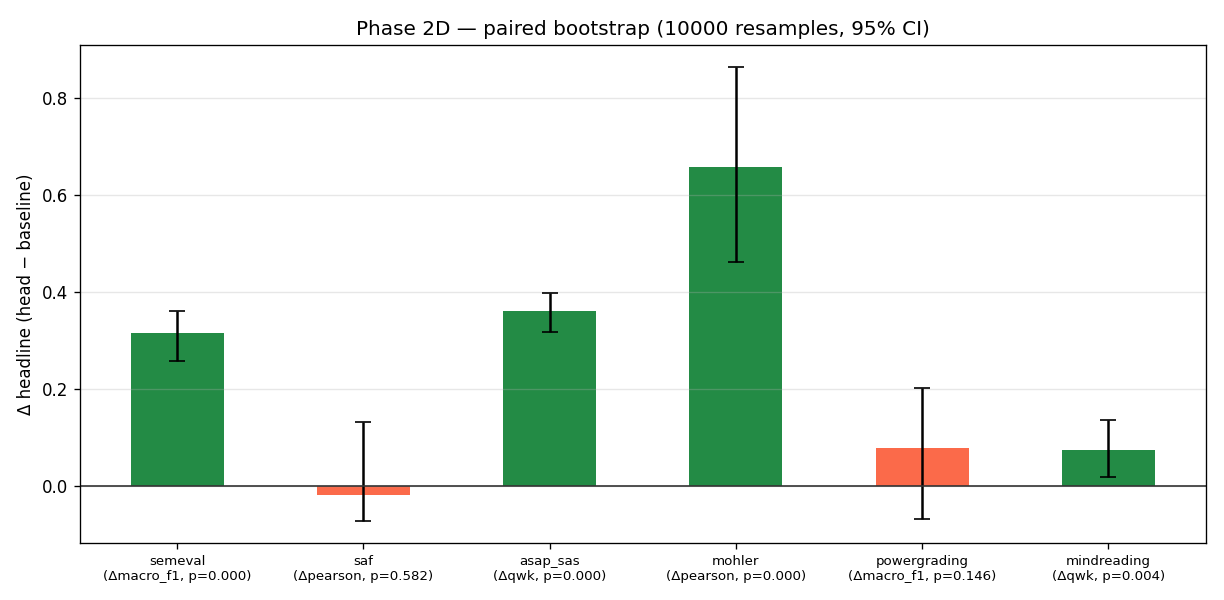
\includegraphics[width=.85\linewidth]{phase2d_significance.png}
\caption{Per-dataset $\Delta$ with cluster-bootstrap 95\% CIs; colored by
whether the effect survives Holm correction.}
\label{fig:sig}
\end{figure}

\subsection{RQ2: Branch ablations under the honest protocol}
\label{sec:results-ablation}

Table~\ref{tab:ablations} removes or isolates each branch with one fixed,
lightly regularized head (so differences are attributable to features, not
tuning). Three findings. \textbf{(i) Linguistic features are the workhorse
where a reference answer exists or length/style signal is informative}:
removing branch~B costs $-0.109$ macro-F1 on SemEval, $-0.340$ QWK on ASAP-SAS
(where B is the only populated branch), $-0.068$ Pearson on Mohler, and all of
MIND-CA's skill. \textbf{(ii) The semantic and rubric branches are
accuracy-light}: $-A$ costs at most $0.020$ anywhere, and $-C$ is within noise
($-0.003$ to $+0.008$); on Powergrading, similarity-only variants
(only-A $0.483$, only-C $0.487$) actually edge out the full model ($0.473$),
suggesting the linguistic branch mildly overfits question style there.
\textbf{(iii) Negation-scope cues deliver small but consistent gains} on five
of six datasets ($-$neg costs $0.009$--$0.029$), validating the
negation-aware preprocessing; the one exception (MIND-CA, $+0.006$) has
answers about mental states where our clause-bounded window is likely too
blunt. Overall: interpretability does not have to be paid for with
accuracy---the faithful rubric branch rides along at no cost---but the
2019-era bi-encoder semantics contribute little, which is precisely the gap
the hybrid arm targets. \TBD{revisit sentence after hybrid run}

\begin{table}[t]
\centering\small
\begin{tabular}{lcccccc}
\toprule
$\Delta$ vs.\ full & SemEval & SAF & ASAP-SAS & Mohler & Powergr. & MIND-CA \\
\midrule
full (abs.) & 0.415 & 0.024 & 0.340 & 0.439 & 0.473 & 0.063 \\
$-$A (semantic) & $-0.014$ & $-0.020$ & 0.000 & $+0.000$ & $-0.002$ & 0.000 \\
$-$B (linguistic) & $-0.109$ & $-0.027$ & $-0.340$ & $-0.068$ & $+0.009$ & $-0.063$ \\
$-$C (rubric) & $-0.003$ & $-0.007$ & 0.000 & $+0.008$ & $-0.001$ & 0.000 \\
$-$neg & $-0.029$ & $-0.021$ & $-0.021$ & $-0.021$ & $-0.009$ & $+0.006$ \\
only-A & $-0.118$ & $+0.008$ & $-0.340$ & $-0.076$ & $+0.010$ & $-0.063$ \\
only-B & $-0.084$ & $+0.022$ & 0.000 & $+0.010$ & $-0.056$ & 0.000 \\
only-C & $-0.128$ & $-0.192$ & $-0.340$ & $-0.105$ & $+0.014$ & $-0.063$ \\
% TODO(after Colab run): add rows "-D (neural)" and "only-D" from the re-run.
\bottomrule
\end{tabular}
\caption{Branch ablations, fixed regularized head, mean over 5 seeds
(\texttt{reports/phase3/ablations.json}); headline metric per dataset as in
Table~\ref{tab:main}. ASAP-SAS and MIND-CA have no reference answer, so
branches A/C are all-NaN and their removal is a no-op by construction.}
\label{tab:ablations}
\end{table}

\begin{figure}[t]
\centering
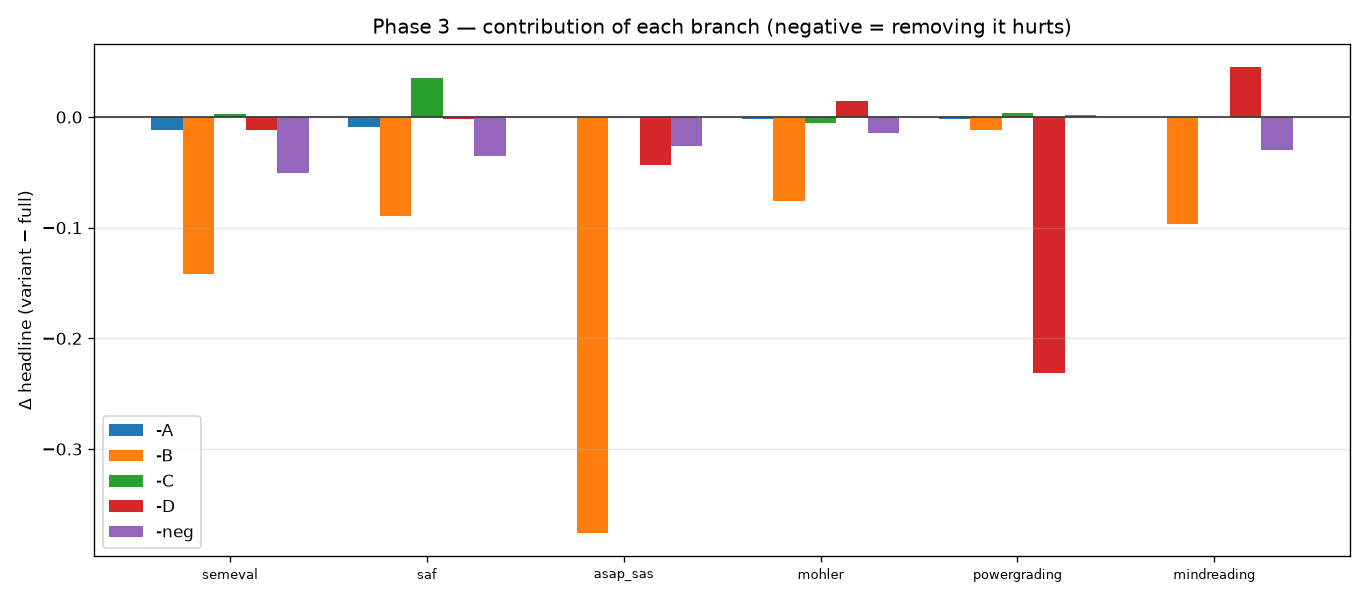
\includegraphics[width=.9\linewidth]{phase3_branch_delta.png}
\caption{Branch ablation deltas vs.\ the full model
(\texttt{reports/phase3/}).}
\label{fig:abl}
\end{figure}

\subsection{RQ3: Explanations---faithful, and validated against humans}
\label{sec:results-xai}

\paragraph{Global attribution sanity.}
Exact TreeSHAP global rankings agree with LightGBM gain rankings (Spearman
$\rho$: SemEval 0.87, SAF 0.65, ASAP-SAS 0.998, Mohler 0.96, Powergrading 0.88,
MIND-CA 0.999), so the explanation layer is not an artifact of one importance
definition.

\paragraph{Faithfulness decomposition.}
For each feature we separate \emph{predictive validity} (Spearman of feature
vs.\ gold score), \emph{model use} (Spearman of feature vs.\ its SHAP
contribution), and \emph{sign consistency} (fraction of items where the SHAP
sign matches the feature's deviation from its median). On Mohler, the rubric
branch has the highest predictive validity of the three branches
($\rho{=}0.34$ vs.\ 0.20 linguistic, 0.14 semantic) while receiving little
attribution mass (21\% of global $|$SHAP$|$ vs.\ 72\% linguistic)---i.e., the
rubric signals are \emph{valid but under-used} by the accuracy-optimal model.
Combined with the $-C\!\approx\!0$ ablation, this yields the paper's central
interpretability finding: \textbf{concept-coverage explanations can be reported
to teachers at essentially zero accuracy cost, but they do not (yet) buy
accuracy}---the head can reconstruct their information from cheaper lexical
signals.

\paragraph{Concept-level attribution.}
Reconstructing per-concept coverage (each reference sentence a concept,
covered iff max similarity $\ge\tau$) yields teacher-style explanations of the
form ``covered $c_1$, $c_3$; missed $c_2$'', e.g., for a SemEval electricity
item, the student's ``positive battery terminal is separated by a gap from
terminal 1'' matches the single reference concept at similarity 0.79 and is
explained as fully covered.

\paragraph{Validation against human gold feedback (SAF).}
SAF ships a human verification verdict per answer
(Correct / Partially correct / Incorrect), which the unified schema discards
and we recover ($n{=}854$ across both test splits). All four interpretable
signals rise strictly monotonically across the verdict classes
(Table~\ref{tab:saf}); semantic cosine is the strongest
($\rho{=}0.255$, AUC${}_{\text{Correct-vs-rest}}{=}0.621$). The effect is
moderate, not decisive---but it is measured against \emph{pre-existing} human
feedback rather than annotations collected to fit the method, and it turns
``the explanations look plausible'' into a quantitative claim.

\begin{table}[t]
\centering\small
\begin{tabular}{lccccc}
\toprule
Signal & Incorrect & Partial & Correct & Spearman $\rho$ & AUC \\
\midrule
rubric coverage@$\tau$ & 0.224 & 0.476 & 0.547 & 0.188 & 0.589 \\
rubric mean max-sim    & 0.399 & 0.488 & 0.521 & 0.198 & 0.599 \\
rubric min max-sim     & 0.306 & 0.347 & 0.391 & 0.139 & 0.575 \\
semantic cosine        & 0.460 & 0.636 & 0.679 & 0.255 & 0.621 \\
\bottomrule
\end{tabular}
\caption{SAF explanation validation: mean signal per human verdict class
($n{=}854$: 63 Incorrect / 304 Partially correct / 487 Correct), Spearman vs.\
the ordinal verdict, and AUC for Correct-vs-rest
(\texttt{reports/phase2f/saf\_validation.json}). All four signals are
monotonic in the human verdict.}
\label{tab:saf}
\end{table}

\begin{figure}[t]
\centering
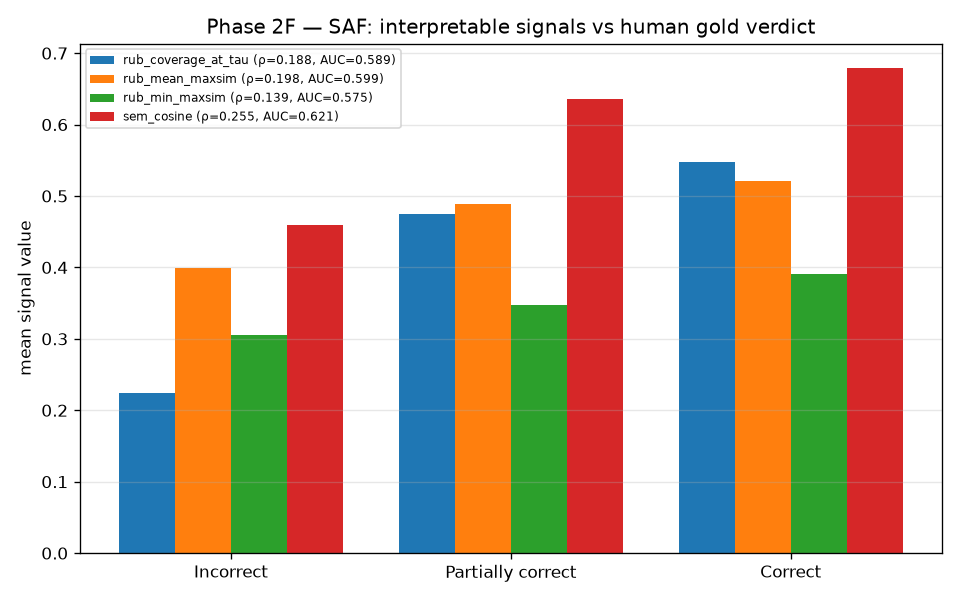
\includegraphics[width=.9\linewidth]{phase2f_saf_validation.png}
\caption{SAF: interpretable signals vs.\ human feedback class
(\texttt{reports/phase2f/}).}
\label{fig:saf}
\end{figure}

\subsection{RQ4a: Calibration and selective prediction}
\label{sec:results-robust}

On SemEval (unseen domains), the raw head is overconfident
(ECE $0.122$); temperature scaling ($T{=}1.35$, fit on a held-out slice of
training data, never on test) halves it to $0.059$
(Figure~\ref{fig:cal}). Powergrading under unseen questions is severely
miscalibrated (ECE $0.613$), and even the optimal temperature ($T{=}5.95$)
only reduces it to $0.334$---quantifying how little the confidence of a
question-memorizing classifier means on new questions. Risk--coverage analysis
supports deferral-based deployment \cite{funayama2020preventing}: routing the
least-confident 20\% of SemEval answers to a human raises accuracy on the
remainder from 0.467 to 0.506, and to 0.575 at 50\% coverage.

\begin{figure}[t]
\centering
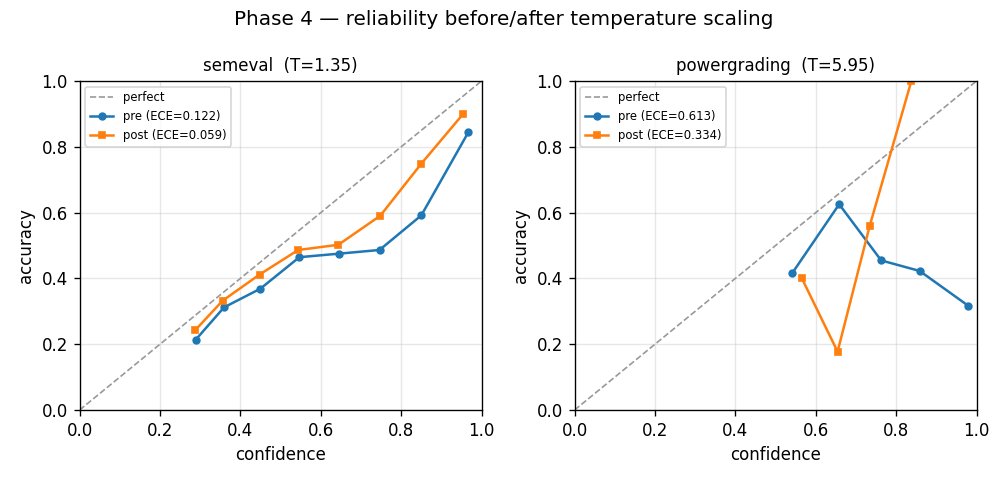
\includegraphics[width=.9\linewidth]{phase4_calibration.png}
\caption{Reliability before/after temperature scaling
(\texttt{reports/phase4\_robust/}).}
\label{fig:cal}
\end{figure}

\subsection{RQ4b: Perturbation robustness}
Three text perturbations probe known failure modes
\cite{filighera2020fooling,ding2020dont}: appending irrelevant filler
(\emph{length pad}), randomly dropping 30\% of tokens (\emph{paraphrase
proxy}), and marking all content tokens as negated (\emph{negation flip}).
Only lexical/negation features are recomputed (semantic and rubric features
held fixed), making the reported sensitivities a conservative bound. As
intended, the grader reacts most strongly to negation flips on SemEval (49\% of
predictions change; mean absolute label shift 0.80)---a grader that ignores
negation would be worse than a brittle one---while the paraphrase proxy changes
18\% of SemEval predictions and systematically lowers Mohler scores (mean
signed shift $-0.24$), exposing the expected lexical-overlap reliance of
branch~B. Length padding shifts predictions on 32\% of SemEval items,
confirming that length features remain a partially open attack surface even
under grouped evaluation.

\subsection{RQ4c: Cross-dataset transfer (LODO)}
\label{sec:results-lodo}

Mapping every dataset to a binary correct/incorrect target and training on
five datasets' shared 31 features while testing on the sixth yields weak and
asymmetric transfer (macro-F1 0.24--0.63): useful signal flows into SemEval
(0.61 macro-F1, AUC 0.68) and Powergrading (0.63, 0.71), SAF is chance-level
(AUC 0.50), and ASAP-SAS \emph{inverts} (AUC 0.27)---features that indicate
correctness elsewhere anti-correlate with it there, plausibly because ASAP's
binarized rubric scores reward length-and-detail patterns that differ from the
overlap-with-reference regime of the other corpora. We report this honest
negative result as a caution against ``train once, grade anywhere'' claims for
feature-based graders; it also mirrors recent findings that cross-domain ASAG
transfer is fragile even for LLMs \cite{meyer2024asag2024}.

\subsection{RQ5: Hybrid arm (pending GPU run)}
\label{sec:results-hybrid}

The three-way comparison---neural-only cross-encoder, feature-only head,
hybrid (features $+$ out-of-fold neural signals)---under identical grouped
folds is fully implemented; the DeBERTa fine-tuning requires a GPU and has not
yet been executed. Table~\ref{tab:hybrid} will report it.
\TBD{Run \texttt{notebooks/02\_neural\_colab.ipynb}, then \texttt{make
neuralfeatures}-dependent re-runs; fill the table; update the abstract,
Sections 2.4, 7.4, 8, and the conclusion.}

\begin{table}[t]
\centering\small
\begin{tabular}{lcccc}
\toprule
Dataset (headline) & Feature-only & Neural-only & Hybrid & $\Delta$ hybrid$-$feat \\
\midrule
SemEval (test\_ud, macro-F1) & $0.427\pm0.005$ & \TBD{} & \TBD{} & \TBD{} \\
SAF (test\_uq, Pearson)      & $0.019\pm0.033$ & \TBD{} & \TBD{} & \TBD{} \\
ASAP-SAS (test\_ua, QWK)     & $0.363\pm0.003$ & \TBD{} & \TBD{} & \TBD{} \\
Mohler (CV, Pearson)         & $0.490\pm0.001$ & \TBD{} & \TBD{} & \TBD{} \\
Powergrading (CV, macro-F1)  & $0.486\pm0.009$ & \TBD{} & \TBD{} & \TBD{} \\
MIND-CA (CV, QWK)            & $0.077\pm0.003$ & \TBD{} & \TBD{} & \TBD{} \\
\bottomrule
\end{tabular}
\caption{\TBD{Hybrid three-way comparison under identical grouped folds
(\texttt{reports/phase\_hybrid/three\_way.json} after the GPU run). Also to
report: share of global $|$SHAP$|$ absorbed by \texttt{neural\_*} (explanation
dilution), and the $-$D ablation row.}}
\label{tab:hybrid}
\end{table}

\subsection{Context against published results}
\label{sec:results-context}

No number in this paper is split-, metric-, and corpus-matched to a published
result, so we make no head-to-head claims: our Mohler is the 21-question
ASAG2024 subset (published Pearson $\sim$0.52 refers to the 80-question 2011
corpus \cite{mohler2011learning}), and our ASAP-SAS covers 4 of 10 prompts
(published neural QWK of 0.72--0.73 refers to all ten
\cite{riordan2017investigating}). Our SemEval headline is the hardest split
(unseen domains); published 5-way macro-F1 figures are typically reported on
unseen answers. We provide our unseen-answer numbers (0.508 macro-F1) to
enable future split-matched comparison, and release per-item predictions.

\section{Discussion}
\label{sec:discussion}

\paragraph{What the audit means for the field.}
The single largest determinant of a reported ASAG number on
no-official-split corpora is not the model but \emph{whether questions span
folds}. Under the leaky protocol, question identity alone is a
top-tier ``model'' (Table~\ref{tab:leakage}). This has two practical
consequences: published stratified-CV results on Mohler/Powergrading-style
corpora should be read as seen-question upper bounds, and new-dataset authors
should ship grouped or unseen-question splits (as SemEval and SAF already do).
The cluster bootstrap is the inferential counterpart: on 20-question corpora,
answer-level CIs are illusions of precision.

\paragraph{What carries accuracy, honestly.}
After leakage is removed, hand-crafted linguistic features still carry the
model; 2019-era bi-encoder semantics add little; and the rubric branch adds
explanation without accuracy. We consider the last point a feature, not a
failure: the coverage signals are valid (they track grades and human
verdicts), so the accuracy-optimal tree simply prefers cheaper correlates.
Whether a \emph{stronger} semantic signal changes this hierarchy is exactly
RQ5. \TBD{one paragraph on the hybrid outcome}

\paragraph{Deployment posture.}
The full system is CPU-only, trains in minutes, is NaN-robust across schema
variation, exposes exact attributions, and its confidence can be temperature-
corrected and thresholded for deferral. In an era of LLM graders with known
leniency and reliability concerns \cite{chamieh2024llms,ferreiramello2025gpt4},
an auditable local grader with quantified unseen-question behavior is a
practical alternative for institutions that must justify grades.

\section{Error Analysis}
\label{sec:error}

On SemEval unseen domains (exact accuracy 46.5\%), the dominant confusion is
\texttt{partially\_correct\_incomplete} predicted as \texttt{correct} (524 of
986 partials; class F1 0.267)---overlap features cannot reliably distinguish
``mentions the right concept'' from ``mentions it completely'', which is
precisely the granularity the rubric branch was designed for and where a
cross-encoder should help most. The second confusion,
\texttt{irrelevant}$\rightarrow$\texttt{correct} (490 of 1{,}222; F1 0.350),
reflects topically-related but non-responsive answers defeating
bag-of-similarity features. \texttt{contradictory} recall is 0.213: negation
cues alone under-detect contradiction, consistent with the small-but-real
$-$neg ablation. The class-frequency skew matters too: \texttt{non\_domain}
has 20 test items (F1 0.625 on trivial support). On Mohler, the perturbation
analysis shows score under-prediction under token drop ($-0.24$ signed),
confirming recall-oriented overlap reliance. These patterns jointly predict
where the hybrid should pay: partial-vs-correct boundaries and
contradiction detection. \TBD{verify prediction post-run}

\section{Threats to Validity}
\label{sec:threats}

\paragraph{Internal.} HPO for k-fold datasets uses inner CV on training rows;
a full nested-CV protocol was not run (documented mild optimism; the tuned-vs-
default gaps in Table~\ref{tab:main} bound its size). Significance point
estimates use seed-42 predictions; 5-seed stds are reported and are an order
of magnitude smaller than bootstrap CIs. Perturbation results recompute only
lexical/negation features (conservative) and are single-run point estimates.
\paragraph{Construct.} Reference sentences are a rubric \emph{proxy}, not
authored rubrics; coverage@$\tau$ uses one fixed $\tau{=}0.5$ (untuned by
design). The unified binary target in LODO imposes a midpoint threshold on
ordinal/continuous scales. \paragraph{External.} English only; short answers
only; Mohler and ASAP-SAS are subsets of their original corpora; SAF test-UQ
has five questions, so its unseen-question estimate is high-variance.
\paragraph{Statistical.} With 11--31 questions per corpus, cluster-bootstrap
CIs are wide by construction; we prefer honest width to item-level optimism.

\section{Limitations}
\label{sec:limitations}

(1)~The semantic branch uses a lightweight 2019-era bi-encoder; its weak
contribution is a statement about that encoder, not about semantics---the
pending DeBERTa arm addresses this directly. (2)~The rubric proxy degenerates
for single-sentence references. (3)~No human study evaluates whether the
concept-coverage explanations are \emph{useful} to teachers; we validate
alignment with human verdicts, not pedagogical utility. (4)~No LLM baseline is
included; the protocol applies to LLM graders unchanged and such a row is
planned. (5)~Runtime/memory profiles, learning curves, and a negation-window
sensitivity analysis are not yet reported. (6)~Datasets are modest in size and
the number of questions per corpus (11--252) bounds the precision of any
unseen-question estimate.

\section{Future Work}
\label{sec:future}

Immediate: execute the DeBERTa hybrid (RQ5) and the $-$D/only-D ablations;
add a zero-shot LLM row under the identical protocol; report runtime and
learning curves. Near-term: rank-consistent ordinal heads (CORAL/CORN
\cite{cao2020coral,shi2023corn}), which to our knowledge remain unapplied in
ASAG; widening ASAP-SAS to all ten prompts and Mohler to the full 2011 corpus
for split-matched comparison; a teacher-facing user study of concept-coverage
explanations. Longer-term: multilingual extension (SAF is bilingual) and
integrating the audit into dataset releases as a standard reporting artifact.

\section{Conclusion}
\label{sec:conclusion}

We presented a leakage-aware evaluation of interpretable ASAG across six
heterogeneous datasets. Question-level leakage inflates the still-common
stratified-CV protocol by up to 38 macro-F1 points, and a
question-identity-only control model explains the inflation; grouped
leave-questions-out CV with cluster-bootstrap significance gives the honest
picture, in which the fusion head beats its controls on four of six datasets.
Hand-crafted linguistic features remain the accuracy workhorse; rubric
concept-coverage explanations are faithful, align monotonically with human
gold feedback on SAF, and cost no accuracy; calibration and deferral analyses
show what it takes to deploy such a grader responsibly. The framework---
grouped folds, shortcut controls, cluster bootstrap, explanation
validation---applies unchanged to transformer and LLM graders, and the pending
DeBERTa-as-feature arm will test whether stronger semantics change the
accuracy hierarchy without sacrificing exact attributions.
\TBD{final sentence after hybrid run}

\section*{Reproducibility and Data Availability}
All code, unified splits (including materialized fold assignments), feature
dictionaries, and every report JSON quoted in this paper are released at
\TBD{repository URL}. Raw datasets are not redistributed; download scripts
with checksums and license notes are provided. Global seed 42; 73 unit tests
cover the schema, split, feature, metric, and head contracts.

\bibliographystyle{plain}
\bibliography{references}

\appendix

\section{Tuned hyperparameters}
\label{app:hpo}
Optuna TPE, 40 trials per dataset, seed fixed; search space: learning rate
$[0.005, 0.3]$ (log), leaves $[15, 255]$, estimators $[100, 800]$, child
samples $[5, 80]$, subsample and column subsample $[0.6, 1.0]$,
$\ell_1/\ell_2$ $[10^{-3}, 10]$ (log).

\begin{table}[h]
\centering\small
\begin{tabular}{lcccccccc}
\toprule
Dataset & lr & leaves & estim. & child & subsamp. & colsamp. & $\ell_1$ & $\ell_2$ \\
\midrule
SemEval      & 0.088 & 114 & 300 & 80 & 0.906 & 0.691 & 9.94 & 0.23 \\
SAF          & 0.096 & 23  & 350 & 17 & 0.927 & 0.807 & 0.07 & 0.72 \\
ASAP-SAS     & 0.023 & 35  & 750 & 41 & 0.832 & 0.904 & 0.64 & 1.22 \\
Mohler       & 0.015 & 115 & 350 & 74 & 0.636 & 0.893 & 1.66 & 0.02 \\
Powergrading & 0.229 & 231 & 650 & 48 & 0.790 & 0.749 & 5.18 & 5.86 \\
MIND-CA      & 0.146 & 49  & 700 & 52 & 0.785 & 0.752 & 0.80 & 0.33 \\
\bottomrule
\end{tabular}
\caption{Per-dataset tuned LightGBM parameters
(\texttt{reports/phase2d/results.json}).}
\label{tab:hpo}
\end{table}

\section{SemEval per-class performance (unseen domains)}
\label{app:confusion}
Per-class F1 (support): correct 0.633 (1{,}917); non\_domain 0.625 (20);
irrelevant 0.350 (1{,}222); partially\_correct\_incomplete 0.267 (986);
contradictory 0.233 (417). Top confusions: partial$\rightarrow$correct (524),
irrelevant$\rightarrow$correct (490), irrelevant$\rightarrow$partial (279).
Full confusion matrices for all datasets:
\texttt{reports/phase3/error\_analysis.json}.

\end{document}
